\documentclass[12pt]{article}

\usepackage{graphicx}
\usepackage{fullpage}
\usepackage[utf8]{inputenc}
\usepackage[brazil]{babel}
\usepackage{amsmath}

\begin{document}

\begin{center}
\Large{DCC04 -- Linear and Binary Search}
\end{center}

\vspace{1cm}

\noindent
Nome: \rule{8cm}{0.01in} \ Matr\'{i}cula: \rule{3cm}{0.01in}

\vspace{1cm}

%%%%%%%%%%%%%%%%%%%%%%%%%%%%%%%%%%%%%%%%%%%%%%%%%%%%%%%%%%%%%%%%%%%%%%%%%%%%%%%%

\begin{enumerate}

\item Define a sorted $M\times N$ matrix $m$ as follows:
\begin{enumerate}
\item For any $0 \leq i < M$ and $1 \leq j < N$, $m[i, j] > m[i, j-1]$
\item For any $1 \leq i < M$ and $0 \leq j < N$, $m[i, j] > m[i-1, j]$
\end{enumerate}
An example can be seen below:

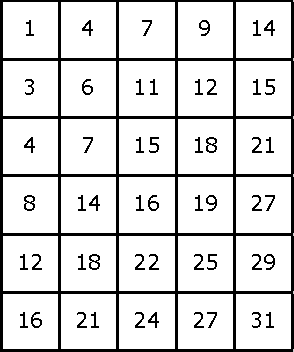
\includegraphics[scale=1]{images/sortedMatrix}

Considering this definition of a sorted matrix, answer the questions below:

\begin{enumerate}
\item What is an efficient algorithm to find any element in this matrix?

\vspace{1cm}

\item What is the asymptotic complexity of your algorithm?

\vspace{1cm}

\item How many comparisons does your algorithm carry out to find if $6$
is in the example matrix?

\vspace{1cm}

\item How many comparisons does your algorithm carry out to find that $5$
is not in the example matrix?
\end{enumerate}

\newpage

\item In programming languages like C or Java, integer arithmetics has
{\em wrapping semantics}.
That means that the addition of two large integers might yield a small
number.
The opposite is also true: the addition of two small numbers (which have negative
sign) might produce a positive number.
From this observation, implement an efficient algorithm that finds the
largest integer in C.
You cannot use any bit-wise operation, or any pre-defined library, such as
\texttt{limits.h}.

\vspace{7cm}

\item Implement a binary search in a contiguous array that receives three
arguments: an integer $e$, an array $v$, and the number $n$ of elements in
$v$.
Your algorithm mush return the index $i$ of $v$ that contains either $e$, or
the element that is the closest of $v$.

\end{enumerate}

\end{document}
